\documentclass[12]{article}

\usepackage{geometry}
\usepackage{amsmath, amsthm, amssymb}
\usepackage{graphicx}
\usepackage{tikz}
\usepackage{booktabs} % See the package documentation for guidelines on formal tables: https://ctan.org/pkg/booktabs
\usepackage{verbatim} % Used to typeset, for example, code snippets or pseudo-code for algorithms.
\usepackage{dsfont} % Extra fontset for helpful mathematics symbols, e.g. \mathds{1}
\usepackage{etoolbox} % Used to allow boolean variables for use in the title page
\usepackage{import}
\usepackage{lipsum}
\usepackage{subcaption}
\usepackage{float}
\usepackage{enumitem}
\usepackage{tabularx}
\usepackage{array}
\usepackage{pdfpages}
\usepackage{mathtools}
\usepackage{hyperref}
\newcolumntype{C}[1]{>{\centering\arraybackslash}m{#1}}

\newcommand{\R}{\mathbb{R}}
\newcommand{\Q}{\mathbb{Q}}
\newcommand{\C}{\mathbb{C}}
\newcommand{\N}{\mathbb{N}}
\newcommand{\Z}{\mathbb{Z}}
\newcommand{\T}{\mathbb{T}}
\newcommand{\cA}{\mathcal{A}}
\newcommand{\cB}{\mathcal{B}}
\newcommand{\cD}{\mathcal{D}}
\newcommand{\cP}{\mathcal{P}}
\newcommand{\cM}{\mathcal{M}}
\newcommand{\abs}[1]{\left\lvert #1 \right\rvert}
\newcommand{\norm}[1]{\left\lVert #1 \right\rVert}
\newcommand{\set}[2]{\left\{#1 \ : \ #2\right\}}
\newcommand{\conv}[1]{\underset{#1}\longrightarrow}
\newcommand{\Mod}[1]{\ (\mathrm{mod}\ #1)}
\newcommand{\Supp}[0]{\ \mathrm{Supp}\ }
\DeclarePairedDelimiter\ceil{\lceil}{\rceil}
\DeclarePairedDelimiter\floor{\lfloor}{\rfloor}
\DeclareMathOperator{\lcm}{lcm}
\newcommand{\Cross}{\mathbin{\tikz [x=1.4ex,y=1.4ex,line width=.2ex] \draw (0,0) -- (1,1) (0,1) -- (1,0);}}

\newcommand\restr[2]{{% we make the whole thing an ordinary symbol
		\left.\kern-\nulldelimiterspace % automatically resize the bar with \right
		#1 % the function
		\vphantom{\big|} % pretend it's a little taller at normal size
		\right|_{#2} % this is the delimiter
}}
% Custom math operators (analogous to \lim, \sup, etc).
\DeclareMathOperator{\id}{id}
\DeclareMathOperator{\subspan}{span}
\DeclareMathOperator{\sgn}{sgn}
\DeclareMathOperator{\diam}{Diam}
\DeclareMathOperator{\mult}{mult}

\newtheorem{thm}{Theorem}[section] % Numbering is impacted by [chapter]; could do [section] or [subsection] also.
\newtheorem{lem}{Lemma} % The [thm] argument says to number Lemma in sequence with Theorem.
\newtheorem{prop}[thm]{Proposition}
\newtheorem{cor}[thm]{Corollary}
\newtheorem{conj}[thm]{Conjecture}
\newtheorem{question}{Question}
% These environments are unnumbered and will not count toward the numbering.
%\newtheorem*{question}{Question}
\newtheorem*{answer}{Answer}
\newtheorem*{conjecture}{Conjecture}
\newtheorem*{claim}{Claim}
% These environments are definitions; they have a different style (bold label, standard font).
\theoremstyle{definition}
\newtheorem{defn}[thm]{Definition} % These definitions are also numbered in sequence with Theorem.
\newtheorem{eg}{Example}
\newtheorem{rem}[thm]{Remark}
\newtheorem{obs}{Observation}

\title{ \vspace{-3cm} Ph.D. Working Notes }
%\author{Tao Gaede}

\begin{document}
	\maketitle
	\tableofcontents
	
	\section{Crescent Labelled Trees}
	
	Let $T$ be a tree of order $n$.  A crescent labelling of $T$ is a map $L: E(T) \mapsto \{1,2, \ldots, t\}$, such that the distance multiset of $L(T)$ is of the form $\{d_1^1,d_2^2, \ldots, d_{n-1}^{n-1}\}$.  The diameter of $T$, denoted $\diam(T)$, is the length of the $(u,v)$-path in $T$.  The max degree of $T$ is denoted $\Delta(T)$.  %We use $\ell$ to denote the number of leaves of $T$.
	

\begin{lem}[Basic Diameter Lower Bound]
	Let $t$ be a positive integer.  If $L(T)$ is a crescent labelling of the tree $T$ with weights $\{1,2,\ldots,t\}$, then $\diam(T) \geq \tfrac{n-1}{t}$.
\end{lem}

\begin{proof}
	Since there are at least $n-1$ distinct distances, there is a distance $d$ with value at least $n-1$.  Let $u,v \in V(T)$ such that $d(u,v) = d$, then since $t$ is the max edge weight, this means that the number of edges on a $(u,v)$-path is at least $\tfrac{d}{t} \geq \tfrac{n-1}{t}$.
\end{proof}
	
	
	For a pair of vertices $u,v \in V(T)$, we denote the $(u,v)$-path in $T$ as $P(u,v)$.  Lemma \ref{Lemma-DegreeClasses} below generalizes the observation underlying the maximum degree upper bound of $\sim$ $\sqrt{2n}$.
	
	\begin{lem}\label{Lemma-DegreeClasses}
		Let $T$ be a tree of order $n$.  For every $i \in [1,n-1]$, $M \in V(T)$, and $j \in \mathcal{N}(M)$, define
		$$D_j := \{u \in V(T) \setminus \{M\}: d(u,M) = d_i, j \in P(u,M)\}.$$
		Then distance $2d_i$ occurs with multiplicity at least $\sum_{j < k}^{\deg(M)} |D_j|\cdot |D_k|$.
	\end{lem}

	\begin{proof}
		Let $M \in V(T)$ and $i \in [1,n-1]$.  Since $T$ is a tree, there is always a unique $(u,v)$-path for all $u,v \in V(T)$.  So, for each $u \in D_j$ and $v \in D_k$, the $(u,v)$-path must go through $M$, which means $d(u,v) = d(u,M) + d(M,v) = 2d_i$.  There are $|D_j| \cdot |D_k|$ such $u$ and $v$ pairs, so indeed $2d_i$ has multiplicity at least $\sum_{j < k}^{\deg(M)} |D_j|\cdot |D_k|$. \qedhere
	\end{proof}
	
	Now we apply the lemma to get a condition on crescent labelled trees.
	
	\begin{prop}[Max Multiplicity Condition]
		Let $L(T)$ be a crescent labelling of a tree $T$.  Then for every $i \in [1,n-1]$, $M \in V(T)$, and $j \in \mathcal{N}(M)$, 
		$$\sum_{j < k}^{\deg(M)} |D_j|\cdot |D_k| < n.$$
	\end{prop}
	
	\begin{proof}
		Since $L(T)$ is a crescent labelling of $T$, no distance can have multiplicity greater than $n-1$and $T$ is a tree.  Since $T$ is a tree, it follows by Lemma \ref{Lemma-DegreeClasses} that for each vertex $M \in V(T)$, $i \in [1,n-1]$, $\sum_{j < k}^{\deg(M)} |D_j|\cdot |D_k| < n$. \qedhere
	\end{proof}
	
	Next is a general lemma on $\{1,2,\ldots,t\}$-words containing subwords with $t-1$ consecutive $1s$.
	
	\begin{lem}[Arithmetic Condition]\label{Lemma-ArithmeticCondition}
		Let $k \geq 2t$.  Let $\mathbf{w}$ be a $\{1,2,\ldots, t\}$-word with length $k$.  If $w_{a-t+2} = w_{a-t+3} = \cdots = w_{a} = 1$ for some $a \in \{1,2, \ldots, k\}$, then each value 
		$$1,2, \ldots, \max\biggr\{\sum_{i = 1}^{a}w_i, \sum_{i=a-t+2}^{k}w_i\biggr\}$$ 
		occurs as a partial sum in $\mathbf{w}$.
	\end{lem}
	
	\begin{proof}
		Suppose without loss of generality that $\sum_{i = 1}^{a}w_i \leq \sum_{i=a-t+2}^{k}w_i$.  Then it is sufficient to show that every value $1,2,\ldots, \sum_{i=a-t+2}^{k}w_i$ occurs as a partial sum in $\mathbf{w}$.  Call $w_{a-t+2},w_{a-t+3}, \ldots, w_a$ the \emph{unit segment} of $\mathbf{w}$ and $w_{a+1},w_{a+2},\ldots,w_k$ the \emph{non-unit segment} of $\mathbf{w}$.  We proceed by induction on the number of terms $r$ in the non-unit segment of $\mathbf{w}$.  When $r = 1$, $w_{a+r} \in \{1,\ldots,t\}$, and since the unit segment has $t-1$ 1s, for each $j \in \{1,2,\ldots,t-1\}$, we have the partial sums $j = \sum_{i=0}^{j-1}w_{a-i}$.  Then the values between $w_{a+r}$ and $\sum_{i=a-t+2}^{a+r}w_i$ are of the form $w_{a+r}+ \sum_{i=0}^{j-1}w_{a-i}$.  For the inductive step, the values $1,2,\ldots,\sum_{i=a-t+2}^{a+r-1}w_i$ occur at least once by inductive hypothesis.  We have that $w_{a+r} \in \{1,2,\ldots,t\}$ and the values between $\sum_{i=a+1}^{a+r-1}w_i$ and $\sum_{i=a+1}^{a+r}w_i$ can be obtained from $\sum_{i=a+1-j}^{a+r-1}w_i$ for each $j \in \{1,2,\ldots,t-1\}$.  Then similarly the values between $\sum_{i=a+1}^{a+r}w_i$ and $\sum_{i=a-t+2}^{a+r}w_i$ are $\sum_{i=a+1-j}^{a+r}w_i$ for $j \in \{1,2,\ldots,t-1\}$. \qedhere
	\end{proof}
	
	We now apply this arithmetic lemma to crescent labelled trees to show that when there are many consecutive 1s on a path, the path cannot be too long with many large weight edges.
	
	\begin{prop}
		Let $L(T)$ be a crescent labelling of a tree $T$ with edge weights in $\{1,2,\ldots,t\}$.  Then for every path $P = (v_1v_2,v_2v_3,\ldots,v_{t-1}v_t)$ in $T$ such that $w(v_iv_{i+1}) = 1$ for $i \in \{1,2,\ldots,t-1\}$, it follows that $\max\{d(v_1,u): u \in V(T)\} < n$ and $\max\{d(v_t,u): u \in V(T)\} < n$.
	\end{prop}
	
	\begin{proof}
		Let $T$ be a tree with a path $P$ specified in the proposition statement and $L(T)$ a crescent labelling.  It is sufficient to show that $\max\{d(v_1,u): u \in V(T)\} < n$ since the case for $v_t$ is similar.  Let $u' \in V(T)$ such that $d(v_1,u') = \max\{d(v_1,u): u \in V(T)\}$.  By Lemma \ref{Lemma-ArithmeticCondition}, every distance $1,2,\ldots, d(v_1,u')$ occurs at least once.  Since $L(T)$ is a crescent labelling, there can be at most $n-1$ distinct distances, so $d(v_1,u') < n$ as desired. \qedhere
	\end{proof}
	The implication for when $t=2$ is quite strong since this imposes a max distance condition on vertices incident to edges with weight $1$.
	\begin{cor}
		Let $L(T)$ be a crescent labelling of a tree $T$.  If $t = 2$, then every vertex incident to an edge with weight $1$ has max distance at most $n-1$.
	\end{cor}
	
	%\begin{prop}
	%	Let $L(T)$ be a crescent labelling of a tree $T$.  For every path $P$ of length $t-1$ whose edges all have weight $1$, each end vertex $v \in P$ satisfies 
	%	$$\max\{d(v,u):u \in V(T)\} \leq n.$$
	%\end{prop}
	
	What follows is a basic lemma about trees that may turn out to be useful in case parameterizing by number of leaves becomes sensible.
	
	\begin{lem}[From Chartrand and Lesniak's text ``Graphs and Digraphs" 4th edition]
		Let $T$ be a tree with $n_i$ vertices with degree $i$, where $i \in \{1,2,\ldots,\Delta(T)\}$.  Then $n_1 = n_3 + 2n_4 + 3n_5 + \cdots + (\Delta(T)-2)n_{\Delta(T)} + 2$.
	\end{lem}
	
	\begin{proof}
		Note that $n = \sum_{i=1}^{\Delta(T)}n_i$.  Since $T$ is a tree, 
		$$\sum_{i=1}^{\Delta(T)} in_i  = \sum_{v \in V(T)} \deg(v) = 2(n-1) = 2\biggr(\sum_{i=1}^{\Delta(T)}n_i \biggr) - 2.$$  
		Rearranging gives $2+ \sum_{i=1}^{\Delta(T)} (i-2)n_i = 0.$
	\end{proof}
	
	\begin{cor}
		If $T$ is a tree, then $\sum_{i=3}^{\Delta(T)}(i-2)n_i < n_1$
	\end{cor}
	
	\section{Polynomial Method}
	
	Let $L(G)$ be a crescent labelling of a graph $G$ with corresponding distance multiset $\{d_1^{1},d_2^{2},\ldots,d_{n-1}^{n-1}\}$. Consider the bipartite multigraph $\mathcal{M} := \mathcal{M}(G)$ where $V(\mathcal{M}) = X \cup Y$, where $X$ consists of the distinct distances $d_1,d_2,\ldots,d_{n-1}$ and $Y$ consists of the vertices of $G$, $v_1,v_2,\ldots,v_n$.  For $d_k\in X$ and $v_i \in Y$, an edge $d_kv_i \in E(\mathcal{M})$ is included for every $j \in [n]$ such that $d(v_i,v_j) = d_k$.  Note that since $L(G)$ is a crescent labelling, for each $k \in [n-1]$, $\deg(d_k) = 2k$.  Observe also that the multiset neighbourhood of $v_i$ is the multiset of the $n-1$ distances between $v_i$ and the other vertices in $G$.
		
	We show a variation of a result from Alon (see proof of Theorem 6.1 in \cite{alon}) about the existence of $p$-regular subgraphs of a multigraph whose average degree is very close to its max degree.  If we relax this strong average degree condition, we can still obtain a rather powerful result whereby a subgraph $U$ of $\mathcal{M}$ has vertex degrees in $\{p,2p,3p,4p,5p,6p,7p\} \cap [2(n-1)]$, where $p \in [\tfrac{n}{4},\tfrac{n}{2}]$, which is significant because $\mathcal{M}$ is bipartite and so the structure of $U$ can tell us some things about how the distances relate to the vertices in $G$.  This subgraph $U$ likely can't be too small, since then there would be a vertex $v \in G$ with too many other vertices at some distance $d$ from $v$.  
	
	\begin{rem}
		Relating the size of this $U$ to the structure of $G$ might be a fruitful way to proceed.  For instance, paths require $|U|$ to be quite large (no vertex is at distance $d$ with more than $2$ other vertices for each $d$).  I think stars might be similar in that they require $|U|$ to be rather large.  Perhaps if $p \sim n/4$, or even asymptotically when $p \sim n/2 - (n/2)^{0.525}$ or so, $U$ being large with min degree $p$ forces convergence of crescent labelled trees to paths and stars.  But I admit, I'm not really sure right now what to do when $|U|$ is big.
	\end{rem}
	
	
	%The key result here is Corollary XX, which says that any crescent labelled graph forces at least one of the vertices to be at distance $d$ from at least $p$ other vertices, where $p \in [\tfrac{n}{4}, \tfrac{n}{2}]$.  
	
	The proof applies Alon's combinatorial nullstellensatz \cite{alon}.  The corollary of the nullstellensatz that we use is as follows:
	
	\begin{lem}[Combinatorial Nullstellensatz]\label{Lemma-CombinatorialNullstellensatz}
		Let $\mathbb{F}$ be a field and let $f \in \mathbb{F}[x_1,x_2,\ldots,x_n]$ be a polynomial such that $\deg(f) = \sum_{i=1}^n t_i$ and the coefficient of $\prod_{i=1}^n x_i^{t_i}$ is non-zero.  Let $S_1,S_2,\ldots,S_n$ be subsets of $\mathbb{F}$ such that $|S_i| > t_i$ for all $i \in [n]$.  Then there exists $(s_1,s_2,\ldots,s_n) \in S_1 \times S_2 \times \cdots \times S_n$ such that $f(s_1,s_2,\ldots,s_n) \neq 0$.
	\end{lem}
	
	\begin{prop}[Variation of Theorem 6.1 in \cite{alon}]\label{Prop-SubgraphNullstellensatzResult}
		Let $p$ be a prime number in $[\tfrac{n}{4},\tfrac{n}{2}]$.  Then $\mathcal{M}(G)$ contains a subgraph $U$ such that for every $u \in V(U)$, $\deg(u) \in \{p,2p, 3p,4p,5p,6p,7p\} \cap [2(n-1)]$.  %In particular, $U$ contains vertices in each part of $\mathcal{M}$, each with degree at least $p$.
	\end{prop}
	\begin{proof}
		We define a polynomial $f$ with degree $|E(\mathcal{M})|$ over $\mathbb{F}_2$, and using the fact that $a^{p-1}$ $\Mod{p}$ $\equiv 1$ for all $a \not\equiv 0 \Mod{p}$, we show the existence of the desired subgraph using the nullstellensatz directly.
		
		Define the polynomial
		$$f(x_e:e \in E(\mathcal{M})) = \prod_{v \in V(\mathcal{M})} \biggr[1 - \Big(\sum_{\substack{e \in E(\mathcal{M})\\ v \in e}}x_e \Big)^{p-1} \biggr] - \prod_{e \in E(\mathcal{M})}(1-x_e).$$
		
		The degree of $f$ is $|E(\mathcal{M})|$ because
		$$|V(\mathcal{M})| (p-1) = (2n-1)(p-1) \leq (2n-1)(\tfrac{n}{2}-1) = n(n-\tfrac{5}{2})+1 < n(n-1) = |E(\mathcal{M})|.$$
		
		Note that the max degree term, $(-1)^{|E(\mathcal{M})|}\prod_{e \in E(\mathcal{M})} x_e$ has a non-zero coefficient. 
		To apply the nullstellensatz, we consider solutions to $f$ of the form $(s_1,s_2,\ldots,s_{|E(\mathcal{M})|}) \in \{0,1\}^{|E(\mathcal{M})|}$ (where $t_i = 1$ for all $i \in [|E(\mathcal{M})|]$).  Thus by Lemma \ref{Lemma-CombinatorialNullstellensatz}, there exists a vector, call it $r=(r_e:e \in E(\mathcal{M}))$, such that $f(r) \neq 0$.  By the definition of $f$, $r \neq 0$ because $f(0) = 0$, so some of its entries are $1$.  This means that the latter product in $f$ vanishes when evaluated at $r$.  The former product in $f$ can be non-zero only when $\Big(\sum_{\substack{e \in E(\mathcal{M})\\ v \in e}}r_e \Big)^{p-1} \equiv 0 \Mod{p}$.  It follows that $r$ corresponds to a subgraph $U$ of $\mathcal{M}(G)$ whose vertex degrees are congruent to $0 \Mod{p}$.  Since $\Delta(\mathcal{M}) = 2(n-1)$ and $r \neq 0$, there exists a vertex $u \in U$ such that $\deg(u) \in \{p,2p, 3p, 4p, 5p, 6p, 7p\} \cap [2(n-1)]$.  Note that since the degrees of the vertices in the neighbourhood of $u$ are all at least $1$, $U$ contains at least one vertex in each part of $\mathcal{M}$ with degree at least $p$. \qedhere
	\end{proof}

	%\begin{cor}
	%	Let $L(G)$ be a crescent labelling of a graph $G$ and $p$ be a prime number in $[\tfrac{n}{4}, \tfrac{n}{2}]$.  Then there exists a vertex $v \in V(G)$ and a distance $d \in \{d_1,d_2,\ldots,d_{n-1}\}$ such that there are at least $p$ other vertices in $G$ at distance $d$ from $v$.
	%\end{cor}
	
	\section{Distance Multiplicities in Unweighted Graphs}
	
	Let $G$ be a tree. Define $T(G)$ to be $G$ without its leaves, and on each vertex $v$ of $T(G)$ assign it a weight equal to the degree of $v$ in $G$, $\deg(v)$.  Define $m(k)$ to be the multiplicity of distance $k$ in a graph $G$.
	
	The following expresses $m(k)$ in terms of the degrees of the vertices of $G$, or equivalently, the vertex weights in $T(G)$.
	
	\begin{lem}[Characterizing Distance Multiplicities in Terms of Vertex Degrees]\label{Lemma-CharacterizingMultiplicityInTermsOfDegrees}
		It holds that $m(1) = |E(G)|$, $m(2) = \sum_{v \in V(G)} {\deg(v) \choose 2}$, and when $3 \leq k \leq \diam(G)$, 
		$$m(k) = \sum_{\substack{\{x,y\} \subset T(G) \\ d(x,y) = k-2}} (\deg(x)-1)(\deg(y)-1).$$
	\end{lem}

	\begin{proof}[Proof sketch]
		The cases $k = 1$ and $k=2$ are straightforward and no distance can be larger than the diameter of $G$.  Suppose $3 \leq k \leq \diam(G)$.  Let $x,y \in T(G)$ where $d(x,y) = k-2$ and let $P(x,y)$ be the unique path of length $k-2$ between $x$ and $y$.  There are $\deg(x)-1$ and $\deg(y)-1$ neighbours of $x$ and $y$ in $G$ that are not in $P(x,y)$.  Let $w$ be such a neighbour of $x$ and $z$ such a neighbour of $y$.  Then the unique $(w,z)$-path contains $P(x,y)$ and has length $k$.  Thus $d(w,z) = k$ and there are $(\deg(x)-1)(\deg(y)-1)$ such pairs.  So, each pair $x,y \in T(G)$ satisfying $d(x,y) = k-2$ contributes a multiplicity for $k$ in $G$ of $(\deg(x)-1)(\deg(y)-1)$.  
		
		It is because $G$ is a tree that this method counts all instances of distance $k$; if $G$ has a cycle, then some distances can be over counted and this sum is an upper bound for $m(k)$. \qedhere
	\end{proof}
	
	\subsection{Conjectures}
	
	\begin{conj}
		Let $d$ be the largest distance that attains maximum multiplicity in a tree $T$.  Then for every $i \in \{d, d+1, \ldots, \diam(T)-1\}$, $m(i) \geq m(i+1)$.
	\end{conj}

	\begin{rem}
		I suspect it is possible to prove this by induction on the path lengths $k$.  That is, every path of length $k+1$ corresponds to at least $1$ distinct path of length $k$.  But I think things get a bit tricky because somehow the maximality of $d$ needs to come into play.
	\end{rem}

	\begin{rem}
		\textbf{There are counter-examples to the related claim} that $m(i) \geq m(i-1)$ for all $i \in \{d,d-1,\ldots,2\}$.
	\end{rem}

	The remaining conjectures are all about upper bounding $m(d)$.  The following proposition handles the lower bound.
	
	\begin{prop}\label{Proposition-Minimizing-m(d)-to(n-1)}
		Let $d$ be the largest distance with max multiplicity in a tree $T$.  If $1 \leq d \leq \lceil \frac{n}{3} \rceil$, then $m(d) \geq n-1$.
	\end{prop}

	\begin{proof}
		It is sufficient to construct a tree $T$ such that $m(d) = |E(T)| = n-1$.  Let $u$ be a root vertex.  Append two paths $X$ and $Y$ of length $d-1$ to $u$. Then for the remaining $n-2(d-1)-1$ vertices, append them as a length $n-2(d-1)-1$ path to $u$.  There are $3(d-1)$ distinct paths of length $d$ with endpoints in $X \cup Y$.  There are $n-2(d-1)-d$ paths of length $d$ with endpoints in $V(T) \setminus (X \cup Y)$. 
		
		Altogether, there are $n-2d+2-d + 3d-3 = n-1$ paths of length $d$ in $T$.  Note that since $d \leq \ceil{n/3}$, 
		$$n-2(d-1)-d \geq n-3\ceil{n/3}+2 = \begin{cases}
			0, \text{ if } n \equiv 1 \Mod{3}	\\
			1, \text{ if } n \equiv 2 \Mod{3},
		\end{cases}$$ and in either case, $m(d) = n-1$.  Observe that in fact $m(1) = m(2) = \cdots = m(d) = n-1$. \qedhere
	\end{proof}
	
	\begin{eg}
		Figure \ref{Figure-ExtremalTreeExampleMinimizingMultiplicity} shows a tree with maximum multiplicity $m(d) = n-1$ where $d=6$ is the largest distance with max multiplicity and $n = 20$.
		\begin{figure}[h]
			\centering
			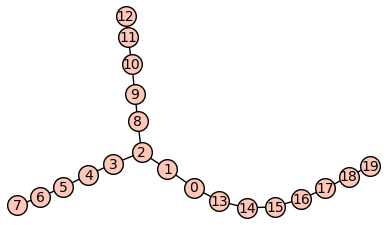
\includegraphics[scale=0.65]{ExtremalTreeExample3(min).png}
			\caption{Extremal tree example minimizing $m(d)$.}\label{Figure-ExtremalTreeExampleMinimizingMultiplicity}
		\end{figure}
	\end{eg}

	\begin{rem}
		Below I conjecture that $d \leq \ceil{n/3}+2$.  I have not yet looked for extremal trees that minimize $m(d)$ when $d \in \{\ceil{n/3}+1, \ceil{n/3}+2\}$.
	\end{rem}
	\newpage
	\begin{conj}
		Let $d$ be the largest distance with max multiplicity in a tree $T$.  
		\begin{enumerate}
			\item If $d \leq C_1\frac{n}{3} + C_2$ and even, then $m(d) \leq (3-a-b)\lceil \frac{r}{3} \rceil \lfloor \frac{r}{3} \rfloor + \lfloor \frac{r}{3} \rfloor^{2a} \lceil \frac{r}{3} \rceil^{2b}$, where $r = n-\tfrac{3}{2}d+2$ and 
			$$(a,b) = \begin{cases}
				(1,0), \text{ if } r \equiv 1 \Mod{3}	\\
				(0,1), \text{ if } r \equiv 2 \Mod{3}	\\
				(0,0), \text{ otherwise. }
			\end{cases}$$
			
			\item If $C_1\frac{n}{3} +C_2< d \leq \lceil \tfrac{n}{3} \rceil + 2$, then $m(d) \leq a\lfloor \frac{r'}{4} \rfloor^2 + (2-a)\lceil \frac{r'}{4} \rceil^2 + 2\lfloor\frac{r'}{4} \rfloor \lceil\frac{r'}{4} \rceil$, where $r' = n-d-1$ and 
			$$a = \begin{cases}
				2, \text{ if } r' \equiv 1 \Mod{4}	\\
				1, \text{ if } r' \equiv 2 \Mod{4}	\\
				0, \text{ otherwise. }
			\end{cases}$$
		\end{enumerate}
	\end{conj}
	
	\begin{rem}
		My experimentation suggests that $C_1 \sim 1$ and $-1 \leq C_2 \leq 1$; however, I have not yet examined these values carefully.
	\end{rem}
	
	
	\begin{rem}
		I believe there are $3$ extremal trees that maximize $m(d)$; one unknown when $d \leq C_1\frac{n}{3} + C_2$ and odd, and the other two are described below.  
	\end{rem}
	
	\begin{prop}[Construction 1]\label{Construction-Small-d-Max-Multiplicity}
		
		Refer to Figure \ref{Figure-ExtremalTreeExamples-a} for an example.  When $d \leq C_1\frac{n}{3}+C_2$ and even, do the following:
		\begin{enumerate}
			\item First we use $3(\frac{d}{2} - 1) + 1$ vertices by making $3$ branch paths with length $\frac{d}{2}-1$ from a root vertex $u$.  
			
			\item Let $v,w,x$ be the vertices at the ends of each branch.  
			
			\item For the remaining $n-3(\frac{d}{2} - 1) - 1$ vertices, append them to $v,w,x$ so that the number of leaf neighbours of $v$, $w$, and $x$ differ from one another by at most $1$.
		\end{enumerate}
	\end{prop} 
	

	\begin{rem}
		Trees with large $m(d)$ when $d  \leq C_1\frac{n}{3} + C_2$ often tend to have a triple branching structure.  The structure of $T$ becomes much more constrained the larger $d$ gets, and I think this is probably because it is most common for $d = 2$.  When $d > 2$, then for $m(2) \leq m(d)$ to hold, \textbf{(1)} the degrees of the vertices of $T$ cannot be too high, and \textbf{(2)} there needs to be enough branching in $T$ to ensure enough distinct length $d$ paths.  Somehow the triple branching pattern in Construction 1 satisfies \textbf{(1)} and \textbf{(2)} while also maximizing $m(d)$; but I doubt that this extremal structure is fragile.  That is, I think even when $d$ is odd and $d  \leq C_1\frac{n}{3} + C_2$, an extremal tree has a similar triple branching structure.
	\end{rem}
	

	\paragraph{Construction 2:} Refer to Figure \ref{Figure-ExtremalTreeExamples-b} for an example.  When $d > C_1\frac{n}{3} + C_2$, do the following:
	\begin{enumerate}
		\item Form a path of length $d-4$ and call its leaves $x$ and $y$.
		
		\item Append two vertices $x_1$ and $x_2$ to $x$ and similarly $y_1$ and $y_2$ to $y$.
		
		\item Append the remaining $n-d-1$ vertices to $x_1$, $y_1$, $x_2$, and $y_2$ so that the number of leaf neighbours on each differ from one another by at most $1$.  If $r' \equiv 2 \Mod{4}$, then ensure that both $x_1$ and $y_1$ are each adjacent to $\ceil{r'/4}$ leaves.
	\end{enumerate}

	\begin{eg}
		Figure \ref{Figure-ExtremalTreeExamples} shows examples from Constructions 1 and 2, which are mentioned above.  In Figure \ref{Figure-ExtremalTreeExamples-a}, $n = 20$, $d = 6$, and $m(6) = 56$.  In Figure \ref{Figure-ExtremalTreeExamples-b}, $n = 24$, $d=\lceil \frac{n}{3} \rceil + 2 = 10$, and $m(d) = 42$.
		
		\begin{figure}[h]
			\centering
			\begin{subfigure}{6.5cm}
				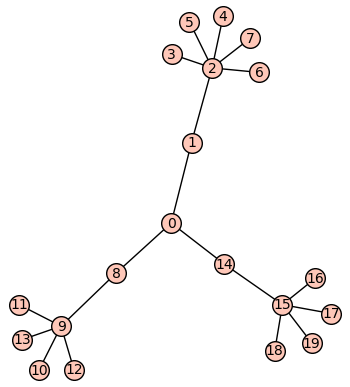
\includegraphics[scale=0.65]{ExtremalTreeExample2.png}
				\caption{Construction 1}\label{Figure-ExtremalTreeExamples-a}
			\end{subfigure}
			\begin{subfigure}{6.5cm}
				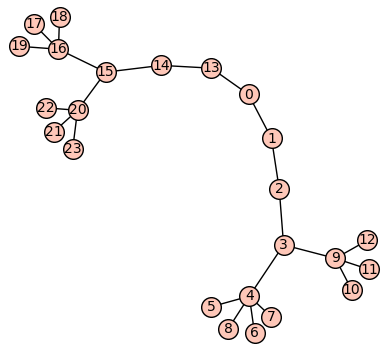
\includegraphics[scale=0.65]{ExtremalTreeExample1.png}
				\caption{Construction 2.}\label{Figure-ExtremalTreeExamples-b}
			\end{subfigure}
			\caption{Extremal tree examples that maximize $m(d)$.}\label{Figure-ExtremalTreeExamples}
		\end{figure}
	\end{eg}

	\begin{conj}
		Let $d$ be the largest distance with max multiplicity.  Then $d \leq \lceil \tfrac{n}{3}\rceil + 2$.
	\end{conj}

	\begin{rem}
		I have not yet found a counter-example to this conjecture.  Please let me know if you find one!  I have searched $n \leq 25$ without finding a CE, but it may well be that $d \leq \ceil{n/3} + C\sqrt{n}$ or something.  If so, then there would probably still be a sensible case division at $d \sim n/3$.
	\end{rem}
	
	
	\iffalse
	\subsection{Constructions}
	
	\begin{prop}
		Let $d$ be the largest distance with max multiplicity.  Then $\min_{T \in \mathcal{T}(n)}m(d) = n-1$.  Let $r = n-3(d/2-1)-1$ and $r' = n-d+1$ and $d$ even.  Then 
		$$\max_{T \in \mathcal{T}(n)}m(d) = \begin{cases}
			\lfloor \tfrac{r}{3} \rfloor(\lfloor \tfrac{r}{3} \rfloor + 2\lceil\tfrac{r}{3} \rceil) & \text{ if } d \leq \tfrac{n}{3}, \text{ and } r \equiv 0,1 \Mod{3}; 	\\
			\lceil \tfrac{r}{3} \rceil(\lceil \tfrac{r}{3} \rceil + 2\lfloor\tfrac{r}{3} \rfloor) & \text{ if } d \leq \tfrac{n}{3}, \text{ and } r \equiv 2 \Mod{3}; 	\\
			
			2\lfloor\tfrac{r'}{4}\rfloor^2 + 2\lfloor\tfrac{r'}{4}\rfloor \lceil\tfrac{r'}{4}\rceil, & \text{ if } d > n/3 \text{ and } r' \equiv 0,1 \Mod{4};	\\
			\lfloor\tfrac{r'}{4}\rfloor^2 + 2\lfloor\tfrac{r'}{4}\rfloor \lceil\tfrac{r'}{4}\rceil + \lceil\tfrac{r'}{4}\rceil^2, & \text{ if } d > n/3 \text{ and } r' \equiv 2 \Mod{4};	\\
			2\lceil\tfrac{r'}{4}\rceil^2 +2\lfloor\tfrac{r'}{4}\rfloor \lceil\tfrac{r'}{4}\rceil, & \text{ if } d > n/3 \text{ and } r' \equiv 3 \Mod{4}.
		\end{cases}$$
	\end{prop}

	\begin{proof}
		When $d \leq \tfrac{n}{3}$, we construct a tree $T$ in two steps.  First we use $3(d/2 + 1) + 1$ vertices by making $3$ branches with length $d-1$ from a root vertex $u$.  Let $v,w,x$ be the vertices at the ends of each branch, respectively.  For the remaining $n-3(d/2 + 1) + 1$ vertices, append them to $v,w,x$ so that the degrees of $v$, $w$, and $x$ differ from one another by at most $1$.  Note that since $d \leq \tfrac{n}{3}$, so $m(2) \leq m(d)$.
	\end{proof}
	\fi
	
	\iffalse
	\section{Crescent Vertices}
	
	Let $v$ be a vertex of a graph $G$.  We say that $v$ is a \emph{crescent vertex} if the multiset of distances from $v$ to every other vertex in $G$ is of the form $\{d_1^{1},d_2^2,\ldots,d_k^{k}\}$ for some $k$.  For example, every vertex in the $4$-cycle $C_4$ is a crescent vertex.  A crescent vertex $v$ has the property that the rest of the vertices can be partitioned into $k$ classes based on the distance from $v$ such that the numbers of vertices in each class is given by a permutation.  We call such a permutation a \emph{crescent permutation}.  For instance, each crescent vertex in $C_4$ induces the crescent permutation $(2,1)$, or $(12)$.  Note that a vertex $v$ is crescent if and only if every other vertex similar to $v$ is crescent, so we are concerned with finding orbits of the given graph that contain crescent vertices.
	
	\begin{question}
		Is $C_4$ the only graph in which every vertex is a crescent vertex?
	\end{question}
	\fi
	
	
	\iffalse
	\section{Hosoya Polynomials}
	
	
	Let $\{d_1^{m_1},d_2^{m_2}, \ldots, d_{k}^{m_k}\}$ be the distance multiset for a graph $G$.  Then the Hosoya polynomial of $G$ is $H_G(x) = \sum_{i=1}^k m_ix^{d_i}$.  Hosoya polynomials appear mainly to just be a reformulation of the distance multiset of $G$, and also $H_G'(1) = \sum_{i=1}^k m_id_i$, which is the sum of all distances in $G$ (often called the Wiener index of $G$).  Note that the Wiener index does not distinguish between which of $d_i$ or $m_i$ is a distinct distance or multiplicity.  Thus for example the Hosoya polynomial for a graph $K$ with $H_K(x) = \sum_{i = 1}^k d_ix^{m_i}$ satisfies $H_K'(1) = H_G'(1)$.  In general, if two distinct graphs $G$ and $K$ have the same Wiener index, does this impose any constraints on the multiplicities of particular distances of $G$ and $K$?  More constraints on $G$ and $K$ are probably needed.  I explore some below.
	
	Suppose $G$ and $K$ have the same order and distances $d_1, d_2, \ldots, d_k$.  Note that if $G$ and $K$ are unlabelled graphs (as opposed to edge-labelled graphs, say), then these distances must be $1, 2, \ldots, k$, where $k = \diam(G) = \diam(K)$.  Represent these distances as a vector $x$, and similarly the multiplicities of $G$, $y = (m_1, m_2, \ldots, m_k)$ and those of $K$, $z = (m_1', m_2', \ldots, m_k')$.  Then if $w(G)$ is the Wiener index of $G$, $xy = xz = w(G)$.  
	
	We can make a matrix $A$ here where $Ax = w \mathbf{1}$.  Sticking with the unlabelled graph case, if the rows of $A$ are multiplicity lists for the distances $1, 2, \ldots, k$ corresponding to graphs with Wiener index $w(G)$, then $\tfrac{Ax}{w(G)} = \mathbf{1}$.  I believe $w(G)$ tells us something about the multiplicity distribution.  In particular, if $w(G)$ is large, then the multiplicities of the large distances should be higher, and if $w(G)$ is small, then the large distance should have smaller multiplicities.  Thus if $H_G'(1) = H_K'(1)$, then we should expect the average difference in multiplicities between $G$ and $K$ to be small; that is, $\tfrac{1}{k}\sum_{i=1}^k |m_i - m_i'|$ should be relatively small.  
	
	
	Here's an attempt:  Let $G$ be a graph with distances $1, 2, \ldots, k$ and respective multiplicities $m_1, m_2, \ldots, m_k$.  Let $y_i$ be the vector $(m_1, m_2, \ldots, m_{i-1}, i, m_{i+1}, \ldots, m_k)$, that is, with $m_i$ swapped for its distance $i$.  Then let $A$ be the matrix with $y_1, y_2, \ldots, y_k$ as row vectors.  Then $Ax = w \mathbf{1}$.  If 
	
	If $x = (1, 2, \ldots, k)$, then I think the average difference $m_i - m_i'$ has to be close to $0$, since otherwise
	
	
	There are 3 main points:
	
	Another construction that tries to minimize mult(d) and mult(2) given that d is the largest distance with maximum multiplicity.  The theme I want to develop here is that if mult(d) = max mult, then mult(2) is very close to mult(d) and minimizing mult(d) can often be achieved by minimizing mult(2) (fewer large degree vertices and smaller max degree).
	Hosoya polynomials seem to provide a way to compare related crescent configuration graph G and H whose multiplicities are a permutation of the distances 1,2, ..., n-1.  Here "related" means (1) G and H have the same Wiener index (sum of all distances), and (2) H has the same distances as G except that some of its distinct distance
	
	
	
	
	A Hosoya polynomial is a degree $k$ polynomial $H(x) = c_0 + c_1x + \cdots + c_kx^k$ in which $c_0 = 0$, and $c_i$ is a positive integer for all $i \in [k]$. This polynomial has the property that its first derivative $H'(x) = \sum_{i=1}^{k}ic_ix^{i-1}$ satisfies $H'(1) = \sum_{i=1}^{k} ic_i$.  Hosoya polynomials were introduced by [so and so] in which $H(x)$ describes the distance multiset of a class of graphs whereby $c_i$ is the multiplicity of distance $i$.  In this graph context where $H(x) = H_\mathcal{G}(x)$ is the Hosoya polynomial for a graph class $\mathcal{G}$, the value $H'(1)$ is the sum of all distances between the vertices in a graph in $\mathcal{G}$; this quantity is called the Wiener index of a graph.  In this section, we make the case that Hosoya polynomials do more than just efficiently represent the distance multiset of a graph, but actually describe a correspondence between graphs with the same Wiener index.
	
	\begin{obs}
		Let $\mathcal{G}$ be a class of edge-weighted graphs of order $n$ with distinct distances $1, 2, \ldots, n-1$ and corresponding Hosoya polynomial $H_\mathcal{G}(x) = \sum_{i=1}^{n-1} \sigma(i)x^{i}$ for some permutation $\sigma$ on $\mathcal{S}_{n-1}$.  Then 
		
		\begin{enumerate}
			\item Each graph in $\mathcal{G}$ is a crescent configuration graph
			\item For each product of disjoint cycles $\tau$ of $\sigma$, the Hosoya polynomial $H_\mathcal{K}(x) = \sum_{i=1}^{n-1} \tau^{-2}\sigma(i)x^{i}$ satisfies $H_\mathcal{K}'(1) = H_\mathcal{G}'(1)$.  
			
			\begin{itemize}
				\item That is, $\tau$ corresponds to a Hosoya polynomial that corresponds to a (\textbf{possibly empty}) class of crescent configuration graphs $\mathcal{K}$ that have the same Wiener index as those in $\mathcal{G}$.  
				\item Essentially, this observation leverages the idea that the Wiener index calculation does not distinguish between multiplicities and distances.  
				\item The permutation structure comes from the fact that we are working with the crescent pattern, which can define a permutation between distinct distances and multiplicities.
				
				\item Note that if $\sigma$ has $b$ disjoint cycles, then there are $2^b$ distinct Hosoya polynomials, each corresponding to a (possibly nonempty) class of crescent configuration graphs related to those in $G$.  Each polynomial can be imagined as a vertex on the hypercube $Q_b$ (each has the same Wiener index and are based on $\sigma$).
				
				\item Note that the polynomial $\sum_{i=1}^{n-1} \sigma^{-1}(i)x^i$ corresponds to the class of crescent configuration graphs with distances and multiplicities equal to the multiplicities and distances, respectively, of those in $\mathcal{G}$.  It might be interesting to compare graphs that manage to have the same Wiener index with their distances and multiplicities swapped.  It's weird to think of distinct distances and multiplicities as interchangeable in this way!
			\end{itemize}
		
			\item Note that $H_G(x) - H_K(x) = \sum_{i=1}^{k}(c_i-r_i)x^{i} = \sum_{i=1}^k c_ix^i - \sum_{j=1}^k$
		\end{enumerate}
		
	\end{obs}

	Note that 
	\begin{align*}
		H_G'(x) - H_K'(x) &= \sum_{i=1}^{k}i(\sigma(i)-\tau^{-2}\sigma(i))x^{i-1}	\\
		&= \sum_{i \in \tau} i(\tau(i)-\tau^{-1}(i))x^{i-1} + \sum_{\substack{i \notin \tau \\ i \in [n-1]}} i(\sigma(i)-\sigma(i))x^{i-1}	\\
		&= \sum_{i \in \tau} i(\tau(i)-\tau^{-1}(i))x^{i-1} + 0	\\
	\end{align*}
	
	So if $\tau = (abc)$, say, then this difference is $a(b-c)x^{a-1} + b(c-a)x^{b-1} + c(a-b)x^{c-1}$.  In particular, when $x=1$, we have $a(b-c) + b(c-a) + c(a-b) = 0$.

	\begin{proof}
		We have that
		\begin{align*}
			H_G'(1) &= H_K'(1)	\\
			\Leftrightarrow \sum_{i=1}^{k} ic_i &= \sum_{i=1}^{k} ir_i	\\
			\Leftrightarrow \sum_{i=1}^{k} i(c_i-r_i) &= 0
		\end{align*}
	
		Note that $H_G'(x) - H_K'(x) = \sum_{i=1}^{k}i(c_i-r_i)x^{i-1}$.
		
		Note that $H_G(x) - H_K(x) = \sum_{i=1}^{k}(c_i-r_i)x^{i}$
	\end{proof}
	\fi
	
	\section{Construction with Large Gap Between Max Multiplicity and $\mathbf{\mult(2)}$}
	
	Let $G$ be a tree of order $n$ and max degree $\Delta$.  Let $d$ be an even distance in $\{2,4,\ldots, n-1\}$ with maximum multiplicity in $G$.  Given $\Delta$ and $d$, the following construction attempts to maximize $\mult(d)$ while minimizing $\mult(2)$.  The idea is to create a tree $G$ where all vertices either have degree $1$ or $\Delta$ and each path of length $d$ has end-vertices with degree $1$ in $G$.  Note that these conditions determine a value of $n = n(d,\Delta)$.  Recall from Proposition \ref{Proposition-Minimizing-m(d)-to(n-1)} and corresponding Figure \ref{Figure-ExtremalTreeExampleMinimizingMultiplicity} that we can minimize $\mult(d)$ at $\mult(2) = n-1$.  Similarly, in the construction from Proposition \ref{Construction-Small-d-Max-Multiplicity}, we had $\mult(2) = \mathcal{O}((\tfrac{n}{3}-\tfrac{3d}{2})^2)$ with $\mult(d) = \mathcal{O}(n^2)$, which are asymptotically equivalent when $d$ is not a function of $n$.  The purpose of the following construction is to show that $\mult(d)$ need not be close to $\mult(2)$; in fact, we will see that it is possible for $\mult(d) = \mathcal{O}(n^2)$ while $\mult(2) = \mathcal{O}(n\Delta)$.
	
	\paragraph{Construction.} Let $d$ and $\Delta$ be positive integers such that $d$ is even.  We construct a graph $G(d,\Delta)$ as follows:
	\begin{enumerate}
		\item Let $r$ be a vertex with neighbours $v_{1},v_{2}, \ldots, v_{\Delta}$.
		
		\item For each $j \in [\Delta]$, identify $v_{j}$ with the root of a $(\Delta-1)$-ary tree with depth $\tfrac{d}{2}-1$.
	\end{enumerate}
	
	\begin{eg}
		Let $(d,\Delta) = (6,4)$.  Then the following tree of order $53$ results from the above construction:
		\begin{figure}[h]
			\begin{center}
				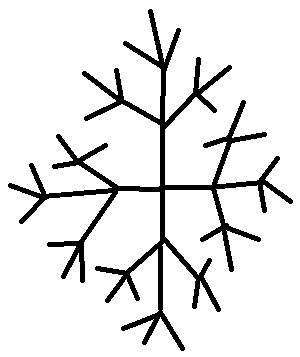
\includegraphics[scale = 0.5]{Delta-ary-tree-example.png}
			\end{center}
			\caption{Example of a tree satisfying $(n,d,\Delta) = (53,6,4)$ where $\mult(2) = 102$ and $\mult(d) = 486$.}
		\end{figure}
	\end{eg}
	
	Let $n_1$ and $n_\Delta$ denote the numbers of vertices with degrees $1$ and $\Delta$, respectively.  We can express both $n_1$ and $n_\Delta$ as functions of $\Delta$ and $d$, and since $n = n_1 + n_\Delta$, we can do the same for $n$.  Note that the eccentricity of the root vertex is $\tfrac{d}{2}$.  We can count the number of vertices by summing the number of vertices at distance $i \in \{0,1, \ldots, \tfrac{d}{2}\}$ from the root.  We have:
	\begin{align*}
		n &= 1 + \Delta + \Delta(\Delta-1) + \cdots + \Delta(\Delta-1)^{\tfrac{d}{2}-1}	\\
		&= 1 + \Delta\sum_{i=0}^{\tfrac{d}{2}-1}(\Delta - 1)^i.
	\end{align*}

	Note that from this we have $n_1 = \Delta(\Delta-1)^{\tfrac{d}{2}-1} = \mathcal{O}(\Delta^{\tfrac{d}{2}})$, and since $n_1 > n_\Delta$, we have $n = n_1 + n_\Delta = \mathcal{O}(\Delta^{\tfrac{d}{2}})$ as well.  The paths with length $d$ always have end-vertices being leaves of $G$ in the $\Delta$ distinct branches from the root of $G$.  There are $(\Delta-1)^{\tfrac{d}{2}-1}$ leaves in each of these $\Delta$ branches, so $\mult(d) = {\Delta \choose 2}(\Delta-1)^{d-2} = \mathcal{O}(\Delta^d)$.  For $\mult(2)$, we sum the ${\Delta \choose 2}$ distinct paths of length $2$ at each of the $1 + \Delta\sum_{i=0}^{\tfrac{d}{2}-2}(\Delta - 1)^i$ non-leaf vertices.  So, $\mult(2) = {\Delta \choose 2}(1 + \Delta\sum_{i=0}^{\tfrac{d}{2}-2}(\Delta - 1)^i) = \mathcal{O}(\Delta^{\tfrac{d}{2}+1})$, and putting all these in terms of $n$, we have $\mult(d) = \mathcal{O}(n^2)$ and $\mult(2) = \mathcal{O}(n\Delta)$, which is quite a large distance.  Thus it is possible to construct trees where the largest distance with maximum multiplicity has multiplicity much larger than the multiplicity of $2$.
	
	The following conjecture reflects the intuition that if distances $2$ and $d = \diam(G)$ have similar multiplicities, then there are few vertices with high degree and little branching.
	
	\begin{conj}
		Let $G$ be a tree with even diameter $d$ where $d$ is the largest distance with maximum multiplicity.  If $\mult(2) \sim \mult(d)$, then there are at most $3$ vertex disjoint paths between the centre and periphery of $G$.
	\end{conj}
	
	\iffalse
	\section{Understanding Distance Multiset Structure Given Graph Symmetry}
	
	The underlying idea here is that we may want to consider ways of partitioning the vertices into classes, whereby we know a lot about the distances between these classes.  The main hypothesis I am proposing is that if we can account for all but $Cn$ of the distances, then we can say a lot about the distance multiset structure of the graph.  For example, we could ignore $C$ pesky vertices that break symmetry, and then use the unbroken symmetry to come up with a nice vertex partition.
	
	What follows is a more detailed example approach.  Observe that if a graph $G$ has a high amount of symmetry, we can sometimes partition $V(G)$ into classes $V_1, V_2, \ldots, V_k$ where the \textit{external} distances between distinct classes $V_i$ and $V_j$ are known, or are even all equal to some small distance multiset $D$.  For instance, the vertices of the graph on $6$ vertices that is a union of a $C_6$ $(v_1v_2v_3v_4v_5v_6v_1)$ and the edge $v_2v_5$ can be partitioned into $\{v_1,v_4\}$, $\{v_2,v_5\}$, and $\{v_3,v_6\}$ whereby the distances between each class is given by the distance multiset $D = \{1^2,2^2\}$.  We have that all but three of the distances are external, which are given by $3$ copies of $D$, $\{1^6,2^6\}$.  The internal distances are $\{1^1,3^2\}$.  In this case, since the external distances are the majority and easily characterized, we can say a lot about the distance multiset of the graph based on external distances only.  For example, the max multiplicity is at least $6$, only distances $1$ or $2$ can have max multiplicity, and since each class has at most ${2 \choose 2} = 1$ edges, the diameter of the graph has to be at most $1 + \max(D) = 3$.
	
	A big picture question is: which graphs have distance multisets that have easy to characterize distance multisets if we ignore distances between only a small number of pesky vertices.  
	
	\paragraph{Trees.} For instance, if we have a tree of order $n$ and we know there are $k$ vertices $v_1, v_2, \ldots, v_k$ such that $\deg(v_i) \geq \ell+1$ and they are all distance $x$ apart from one another, then $\mult(x) \geq {k \choose 2} \ell^2$.  The more general observation is that even if these vertices aren't equidistant, there are at most ${k \choose 2}$ distinct distances that receive multiplicity in multiples of $\ell^2$.
	
	Suppose $n = (k+1)\ell + C$ where there are $k$ vertices with degree at least $\ell + 1$.  Then ${k \choose 2}\ell^2$ of the distances occur between these $k$ stars, and $(k+1)\ell C + {C \choose 2}$ distances involve the $C$ vertices outside the stars.  If $(k+1)\ell = \mathcal{O}(n)$ and $C$ is a constant, then the number of distances involving vertices outside the stars is $\mathcal{O}(n)$.  This means that as $n$ gets big, the distance multiset of the tree is mostly described by the distances between stars, which contribute multiplicity in multiples of $\ell^2$.
	
	For example, suppose $k \sim \tfrac{n-10}{10}$, $\ell = 10$, and $C = 10$.  Then there are around $(n-10)10 + 50 = 10n - 50$ distances involving the $10$ non-star vertices.  There are around $\tfrac{(n-10)^2}{2}$ distances between stars, and they contribute multiplicity in multiples of $\ell^2 = 100$.  I think this means we should expect jumps in multiplicity on the order of something like $\ell^2$.  Put another way, $\ell$ might be relate to the slope of the multiplicity distribution.
	\fi
	
	\newpage
	
	\section{Distance Multisets of Specific Graphs}
	
	\begin{obs}
		Paths of order $n$ have distance multiset $\{1^{n-1},2^{n-2}, \ldots, (n-1)^1\}$.
	\end{obs}
	
	\begin{obs}
		Odd cycles of order $n$ have distance multiset $\{1^n, 2^n, \ldots, \floor{\tfrac{n}{2}}^n\}$.  Even cycles of order $n$ have distance multiset $\{1^n, 2^n, \ldots, (\tfrac{n}{2}-1)^n, (\tfrac{n}{2})^{\tfrac{n}{2}}\}$.
	\end{obs}
	
	\begin{prop}
		The grid graph with dimensions $a$ and $b$ has distance multiset $\{\}$.
	\end{prop}
	
	\begin{proof}
		Let $a$ and $b$ be the dimensions of a grid graph $G_{a,b}$.  Note that the distance of $G_{a,b}$ are the internal distances of $G_{a,b-1}$ and $P_a$ along with the external distances between a $G_{a,b-1}$ and $P_a$.
		
		Let $P_a = (v_1,v_2,\ldots, v_{a})$.  Note for each $i \in [0,\floor{n/2}]$ that $v_i$ and $v_{a-i}$ have the same distances with $G_{a,b-1}$.  We can partition $V(G_{a,b-1})$ into $a$ $P_{b-1}$s, call them $P(1), P(2), \ldots, P(a)$.  Suppose $v_i$ is adjacent to an end-vertex in $P(i)$.  For a given $i \in [0,\tfrac{a}{2}]$, for all $j \in [i,a]$, then the distances between $v_i$ and $P(j)$ are $\{1, 2, \ldots, b-1\} + j-i$; similarly, for all $j \in [1,i-1]$, the distances between $v_i$ and $P(j)$ are $\{1, 2, \ldots, b-1\} + i-j$.
		
		So, the distances $\{1, 2, \ldots, b-1\}$ occur $a$ times, $\{1, 2, \ldots, b-1\}+1$ occur $a-1$ times, and in general $\{1, 2, \ldots, b-1\} + i$ occur $a-i$ times.  Similarly, the distances $\{1, 2, \ldots, b-1\} + a-i$ occurs $i$ times.  So, when $i = 0$, distance $d$ occurs $a$ times...[need to finish].
	\end{proof}

	\begin{prop}
		There does not exist a tree of order $n$ with uniform distance multiplicities.
	\end{prop}

	\begin{proof}
		Let $m$ be the multiplicity of each graph distance in $T$ and $d$ its diameter.  Then ${n \choose 2} = md$.  Since $T$ is a tree, $\mult(1) = n-1$, so $m = n-1$.  Thus $d = \tfrac{n}{2}$.  Let $T_0 = (v_1, v_2, \ldots, v_d)$ be a diametrical path.  Order the vertices of $V(T) \setminus P = (u_1, u_2, \ldots, u_{n-d})$ in a way so that for all $i \in \{1, 2, \ldots, n-d\}$, each graph $T_i$ induced by $P \cup \{u_1, u_2, \ldots, u_i\}$ is connected.  Since $d$ is the diameter, $u_1$ in $T_1$ is adjacent to a vertex in $T_{0}$ with degree $2$; thus both distances $1$ and $2$ in $T_1$ have multiplicity $\tfrac{n}{2}$.  Since $T_i$ is connected, the neighbour of $u_i$ in $T_i$ has degree at least $1$ in $T_{i-1}$, so the multiplicity of distance $2$ in $T_i$ increases by at least $1$ compared to $T_{i-1}$.  So if for some $i \in \{2, 3, \ldots, n-d\}$, the neighbour of $u_i$ in $T_{i-1}$ has degree at least $2$, then $\mult(2) > \mult(1)$ in $T$.  So, the only way for $\mult(2) = \mult(1)$ in $T$ is if every added vertex gets joined with a leaf such that the resulting tree has diameter $d$.  But in this case $T$ has exactly $3$ leaves, which means $T$ has at most $3$ diametrical paths and so $m \leq 3$.  The only solutions are $K_2$ and $K_{1,3}$.
	\end{proof}
	
	\begin{prop}
		The distance multiset of any tree of order $n$ with diameter $d \leq 3$ can be expressed in terms of its degree sequence.
	\end{prop}

	\begin{proof}
		Let $T$ be a tree with diameter $d \leq 4$.  If $d = 2$, then since $T$ is a tree, $\mult(1) = n-1$ and so $\mult(2) = {n \choose 2} - (n-1) = (n-1)(\tfrac{n}{2}-1)$.  Note that $T$ has exactly one vertex $v$ with degree at least $2$, so $\mult(2) = \sum_{u \in V(T)}\deg(u) = \deg(v)$.  If $d=3$, then $\mult(2) = \sum_{u \in V(T)}\deg(u)$ and $\mult(3) = {n \choose 2} - \mult(2) - \mult(1) = {n \choose 2} - \sum_{u \in V(T)}\deg(u) - (n-1)$. \qedhere
	\end{proof}

	\begin{obs}
		Note that the structure of $T$ is necessary to determine $\sum_{u_1u_2 \in E(T)}(\deg(u_1)-1)(\deg(u_2)-1)$.  So for the case when $d=4$, we have $\mult(3) = \sum_{u_1u_2 \in E(T)}(\deg(u_1)-1)(\deg(u_2)-1)$, and so 
		$$\mult(4) = {n \choose 2} - \sum_{u_1u_2 \in E(T)}(\deg(u_1)-1)(\deg(u_2)-1) - \sum_{u \in V(T)}\deg(u) - (n-1).$$
	\end{obs}
	
	\begin{prop}
		Let $T$ be a tree with $m$ distinct multiplicities $m_1, m_2, \ldots, m_m$ such that for $i \in [m]$, there are $x_i$ distances with multiplicity $m_i$.  Then the diameter of $T$ is $d = ...$.
	\end{prop}

	\begin{proof}
		Note that ${n \choose 2} = \sum_{i=1}^m m_ix_i$.  Suppose wlog that $m_1 < m_2 < \cdots < m_m$.  Note that $d = \sum_{i=1}^m x_i \Leftrightarrow x_m = d - \sum_{i=1}^{m-1}x_i$.  Let $x = \sum_{i=1}^{m-1}m_ix_i$ and set $M = m_m$.  Then ${n \choose 2} = x + M(d-\sum_{i=1}^{m-1}x_i)$, so
		\begin{align*}
			{n \choose 2} &= x + Md - M\sum_{i=1}^{m-1}x_i	\\
			\Leftrightarrow d &= \frac{1}{M}\biggr[{n \choose 2} - \sum_{i=1}^{m-1}m_ix_i\biggr] + \sum_{i=1}^{m-1}x_i 	\\
		\end{align*}
	\end{proof}
	
	\newpage
	\begin{thebibliography}{100}
		\bibitem{alon} Alon, N. (1999). Combinatorial Nullstellensatz. Combinatorics, Probability and Computing, 8(1-2), 7-29. doi:10.1017/S0963548398003411
	\end{thebibliography}
	
\end{document}